\documentclass{standalone}
\usepackage{tikz}
\usetikzlibrary{patterns, positioning}


\begin{document}
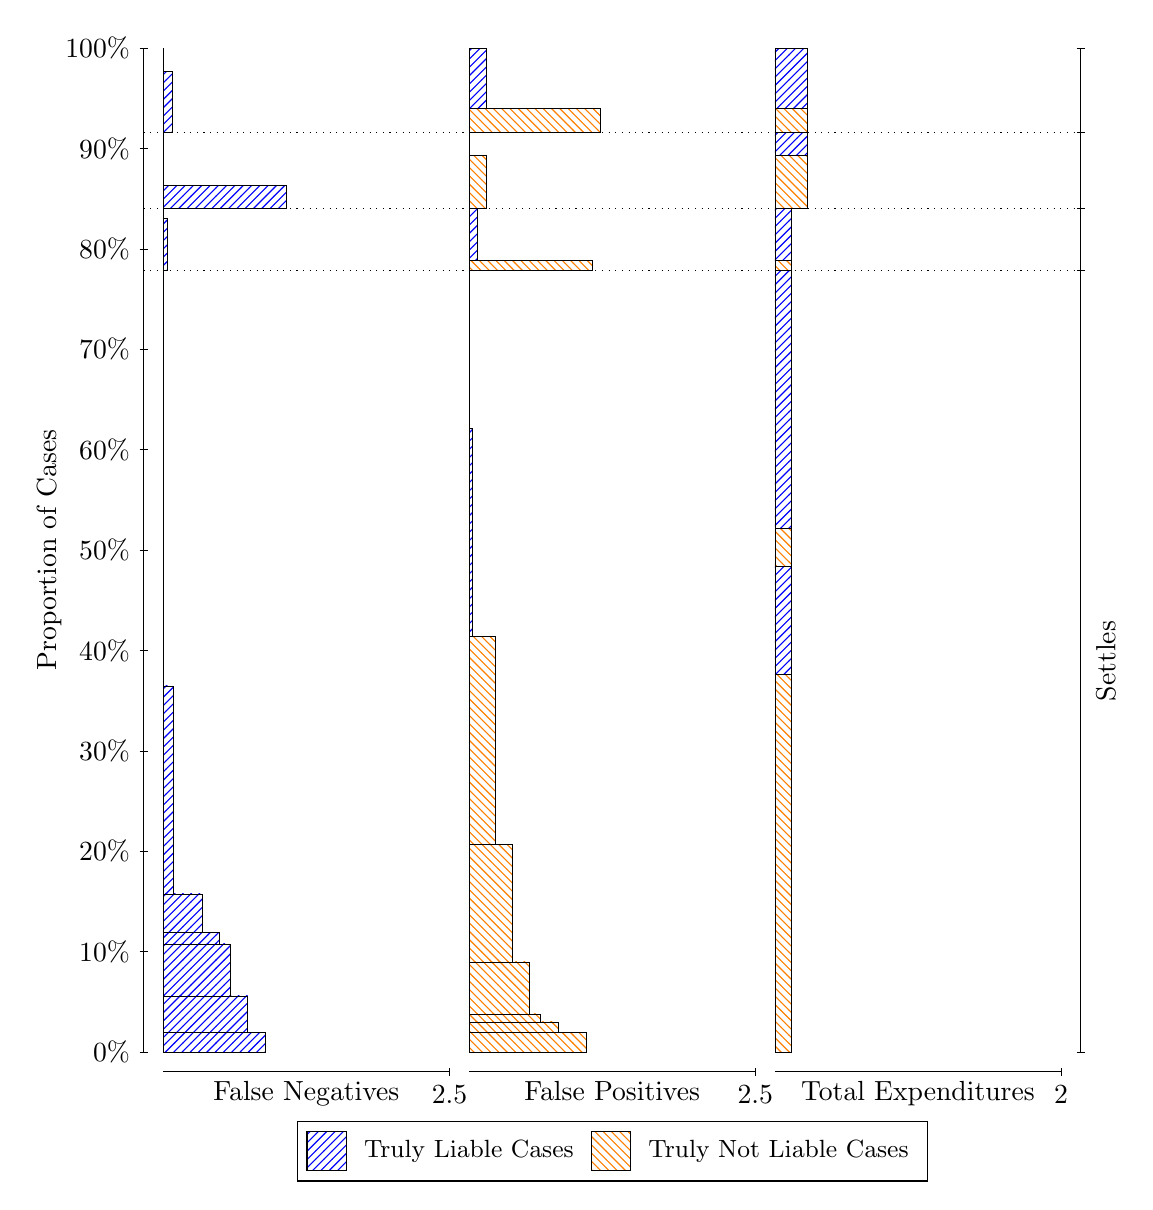
\begin{tikzpicture}
\draw[black, very thin] (1.5,1.75) -- (1.5,14.5);
\node[rotate=90, text=black, anchor=center] at (0.3, 8.125) {Proportion of Cases};
\draw[black, very thin] (1.45,1.75) -- (1.55,1.75);
\node[text=black, anchor=east] at (1.45, 1.75) {0\%};
\draw[black, very thin] (1.45,3.025) -- (1.55,3.025);
\node[text=black, anchor=east] at (1.45, 3.025) {10\%};
\draw[black, very thin] (1.45,4.3) -- (1.55,4.3);
\node[text=black, anchor=east] at (1.45, 4.3) {20\%};
\draw[black, very thin] (1.45,5.575) -- (1.55,5.575);
\node[text=black, anchor=east] at (1.45, 5.575) {30\%};
\draw[black, very thin] (1.45,6.85) -- (1.55,6.85);
\node[text=black, anchor=east] at (1.45, 6.85) {40\%};
\draw[black, very thin] (1.45,8.125) -- (1.55,8.125);
\node[text=black, anchor=east] at (1.45, 8.125) {50\%};
\draw[black, very thin] (1.45,9.4) -- (1.55,9.4);
\node[text=black, anchor=east] at (1.45, 9.4) {60\%};
\draw[black, very thin] (1.45,10.675) -- (1.55,10.675);
\node[text=black, anchor=east] at (1.45, 10.675) {70\%};
\draw[black, very thin] (1.45,11.95) -- (1.55,11.95);
\node[text=black, anchor=east] at (1.45, 11.95) {80\%};
\draw[black, very thin] (1.45,13.225) -- (1.55,13.225);
\node[text=black, anchor=east] at (1.45, 13.225) {90\%};
\draw[black, very thin] (1.45,14.5) -- (1.55,14.5);
\node[text=black, anchor=east] at (1.45, 14.5) {100\%};

\draw[black, very thin] (13.4,1.75) -- (13.4,14.5);
\draw[black, very thin] (13.35,1.75) -- (13.45,1.75);
\node[anchor=west] at (13.35, 1.75) {};
\draw[black, very thin] (13.35,11.679) -- (13.45,11.679);
\node[anchor=west] at (13.35, 11.679) {};
\draw[black, very thin] (13.35,12.459) -- (13.45,12.459);
\node[anchor=west] at (13.35, 12.459) {};
\draw[black, very thin] (13.35,13.432) -- (13.45,13.432);
\node[anchor=west] at (13.35, 13.432) {};
\draw[black, very thin] (13.35,14.5) -- (13.45,14.5);
\node[anchor=west] at (13.35, 14.5) {};

\draw[black, very thin, pattern color=blue, pattern=north east lines] (1.75,1.75) rectangle (3.0398,2.0016);
\draw[black, very thin, pattern color=blue, pattern=north east lines] (1.75,2.0016) rectangle (2.8218,2.4631);
\draw[black, very thin, pattern color=blue, pattern=north east lines] (1.75,2.4631) rectangle (2.6038,3.1234);
\draw[black, very thin, pattern color=blue, pattern=north east lines] (1.75,3.1234) rectangle (2.4585,3.2658);
\draw[black, very thin, pattern color=blue, pattern=north east lines] (1.75,3.2658) rectangle (2.2405,3.7584);
\draw[black, very thin, pattern color=blue, pattern=north east lines] (1.75,3.7584) rectangle (1.8772,6.4006);
\draw[black, very thin, pattern color=orange, pattern=north west lines] (1.75,6.4006) rectangle (1.75,11.679);
\draw[black, very thin, pattern color=blue, pattern=north east lines] (1.75,11.679) rectangle (1.8045,12.335);
\draw[black, very thin, pattern color=orange, pattern=north west lines] (1.75,12.335) rectangle (1.75,12.459);
\draw[black, very thin, pattern color=blue, pattern=north east lines] (1.75,12.459) rectangle (3.3123,12.759);
\draw[black, very thin, pattern color=orange, pattern=north west lines] (1.75,12.759) rectangle (1.75,13.432);
\draw[black, very thin, pattern color=blue, pattern=north east lines] (1.75,13.432) rectangle (1.859,14.201);
\draw[black, very thin, pattern color=orange, pattern=north west lines] (1.75,14.201) rectangle (1.75,14.5);
\draw[black, very thin, pattern color=orange, pattern=north west lines] (5.6333,1.75) rectangle (7.123,2.0016);
\draw[black, very thin, pattern color=orange, pattern=north west lines] (5.6333,2.0016) rectangle (6.7597,2.1332);
\draw[black, very thin, pattern color=orange, pattern=north west lines] (5.6333,2.1332) rectangle (6.5417,2.2345);
\draw[black, very thin, pattern color=orange, pattern=north west lines] (5.6333,2.2345) rectangle (6.3963,2.8948);
\draw[black, very thin, pattern color=orange, pattern=north west lines] (5.6333,2.8948) rectangle (6.1783,4.3863);
\draw[black, very thin, pattern color=orange, pattern=north west lines] (5.6333,4.3863) rectangle (5.9603,7.0286);
\draw[black, very thin, pattern color=blue, pattern=north east lines] (5.6333,7.0286) rectangle (5.6697,9.6708);
\draw[black, very thin, pattern color=blue, pattern=north east lines] (5.6333,9.6708) rectangle (5.6333,11.679);
\draw[black, very thin, pattern color=orange, pattern=north west lines] (5.6333,11.679) rectangle (7.1957,11.803);
\draw[black, very thin, pattern color=blue, pattern=north east lines] (5.6333,11.803) rectangle (5.7423,12.459);
\draw[black, very thin, pattern color=orange, pattern=north west lines] (5.6333,12.459) rectangle (5.8513,13.133);
\draw[black, very thin, pattern color=blue, pattern=north east lines] (5.6333,13.133) rectangle (5.6333,13.432);
\draw[black, very thin, pattern color=orange, pattern=north west lines] (5.6333,13.432) rectangle (7.3047,13.731);
\draw[black, very thin, pattern color=blue, pattern=north east lines] (5.6333,13.731) rectangle (5.8513,14.5);
\draw[black, very thin, pattern color=orange, pattern=north west lines] (9.5167,1.75) rectangle (9.721,6.5442);
\draw[black, very thin, pattern color=blue, pattern=north east lines] (9.5167,6.5442) rectangle (9.721,7.9176);
\draw[black, very thin, pattern color=orange, pattern=north west lines] (9.5167,7.9176) rectangle (9.721,8.402);
\draw[black, very thin, pattern color=blue, pattern=north east lines] (9.5167,8.402) rectangle (9.721,11.679);
\draw[black, very thin, pattern color=orange, pattern=north west lines] (9.5167,11.679) rectangle (9.721,11.803);
\draw[black, very thin, pattern color=blue, pattern=north east lines] (9.5167,11.803) rectangle (9.721,12.459);
\draw[black, very thin, pattern color=orange, pattern=north west lines] (9.5167,12.459) rectangle (9.9254,13.133);
\draw[black, very thin, pattern color=blue, pattern=north east lines] (9.5167,13.133) rectangle (9.9254,13.432);
\draw[black, very thin, pattern color=orange, pattern=north west lines] (9.5167,13.432) rectangle (9.9254,13.731);
\draw[black, very thin, pattern color=blue, pattern=north east lines] (9.5167,13.731) rectangle (9.9254,14.5);
\draw[black, dotted] (1.5,11.679) -- (13.4,11.679);
\draw[black, dotted] (1.5,12.459) -- (13.4,12.459);
\draw[black, dotted] (1.5,13.432) -- (13.4,13.432);
\draw[black, very thin] (1.75,1.5) -- (5.3833,1.5);
\node[text=black, anchor=north] at (3.5667, 1.5) {False Negatives};
\draw[black, very thin] (5.3833,1.45) -- (5.3833,1.55);
\node[text=black, anchor=north] at (5.3833, 1.45) {2.5};

\draw[black, very thin] (5.6333,1.5) -- (9.2667,1.5);
\node[text=black, anchor=north] at (7.45, 1.5) {False Positives};
\draw[black, very thin] (9.2667,1.45) -- (9.2667,1.55);
\node[text=black, anchor=north] at (9.2667, 1.45) {2.5};

\draw[black, very thin] (9.5167,1.5) -- (13.15,1.5);
\node[text=black, anchor=north] at (11.333, 1.5) {Total Expenditures};
\draw[black, very thin] (13.15,1.45) -- (13.15,1.55);
\node[text=black, anchor=north] at (13.15, 1.45) {2};

\node[text=black, centered, rotate=90] at (13.72, 6.7146) {Settles};




\draw (7.449999999999999,1.5) node[draw=none] (baseCoordinate) {};
\begin{scope}[align=center]
        \matrix[scale=0.5, draw=black, below=0.5cm of baseCoordinate, nodes={draw}, column sep=0.1cm]{
            \node[rectangle, draw, minimum width=0.5cm, minimum height=0.5cm, pattern color=blue, pattern=north east lines] {}; &
            \node[draw=none, font=\small, text=black] (B) {Truly Liable Cases}; &
            \node[rectangle, draw, minimum width=0.5cm, minimum height=0.5cm, pattern color=orange, pattern=north west lines] {}; &
            \node[draw=none, font=\small, text=black] (B) {Truly Not Liable Cases}; \\
            };
\end{scope}

\end{tikzpicture}
\end{document}